\chapter{Umsetzung und Ergebnisse}
\label{cha:umsetzung}

%Je nach Art der Arbeit kann diese Kapitelüberschrift auch \glqq Ergebnisse\grqq~lauten, z.~B. bei rein messtechnischen Aufgaben.

%Beschreibung der Umsetzung des zuvor gewählten Vorgehens (theoretische Untersuchung, Erhebungen, Durchführung von Experimenten, Prototypenaufbau, Implementierung eines Prozesses, etc.).

%Verifikation anhand der zuvor erarbeiteten Anforderungen und Validierung in Bezug auf das zuvor gestellte Ziel. Diskussion der Ergebnisse. Spätestens hier auch auf die Zuverlässigkeit der gewonnenen Erkenntnisse eingehen (z.~B. anhand der Genauigkeit von Messergebnissen).
\section{Mechanischer Aufbau des LEGO-Spike-4-Gewinnt-Roboters}


Für die Umsetzung des 4-Gewinnt-Roboters wurde eine mechanische Konstruktion gewählt, die es erlaubt, das Spielfeld zu scannen sowie Chips gezielt in eine Spalte einzuwerfen. Der Aufbau umfasst drei LEGO Spike-Motoren, einen Farbsensor und einen Drucktaster. Im Folgenden werden die einzelnen Komponenten detailliert beschrieben.

\begin{itemize}
	\item \textbf{Horizontalantrieb – Motor D}\\
	Der horizontale Antrieb des Farbsensors erfolgt über Motor D. Dieser ist dafür zuständig, die Spielfeldspalten nacheinander anzufahren. Der Motor ist mit einer Achse verbunden, welche zwei Räder antreiben. Die Bewegung erfolgt in gleichmäßigen Schritten: Eine Drehung um exakt 72 Grad bewegt den Schlitten um eine Spalte weiter. Diese Schrittweite wurde so gewählt, dass sie der Breite einer Spalte im Spielfeld entspricht. Dadurch ist eine exakte Positionierung des Sensors über jeder Spalte möglich, ohne dass zusätzliche Sensoren zur Positionsbestimmung notwendig sind. 
	\item \textbf{Vertikalantrieb – Motor E, Kette und Farbsensor}\\
	 Um das Spielfeld auch in vertikaler Richtung abfahren zu können, ist der Farbsensor an einer Kette montiert. Diese Kette wird durch Motor E angetrieben. Der Sensor ist an einem mittleren Segment der Kette befestigt und fährt beim Drehen der Kette entsprechend auf und ab. Ein Schritt des Motors um etwa 95 Grad bewegt den Sensor um genau eine Spielfeldhöhe weiter. Auf diese Weise können sämtliche sechs Reihen der aktuellen Spalte nacheinander abgescannt werden. Der Sensor wurde dabei so montiert, dass er exakt über der Mitte jedes Feldes positioniert ist, um eine zuverlässige Farberkennung zu ermöglichen. Die Rückwärtsbewegung der Kette erlaubt es, den Sensor wieder nach unten zu fahren.
	\item \textbf{Chipauswerfer – Motor A}\\
	Das Einwerfen des eigenen Spielsteins erfolgt über Motor A. An diesem Motor ist eine Stange montiert, die bei einer vollständigen Umdrehung einen Spielchip aus dem Vorratsmagazin in die gewünschte Spalte stößt. Nach der Auslösung kann ein neuer Chip in die Abschussposition nachrutschen. In der Software ist eine Wartezeit nach dem Auslösen eingebaut, damit der Chip sicher im Spielfeld ankommt, bevor die nächste Aktion beginnt.
	\item \textbf{Startsignal – Drucksensor (Force Sensor)}\\
	Um dem Roboter mitzuteilen, dass der menschliche Spieler seinen Zug abgeschlossen hat, wurde ein Drucksensor verwendet. Dieser befindet sich an der Vorderseite des Roboters. Sobald der Spieler den Sensor leicht berührt, wird ein Signal ausgelöst, das Prozess startet. 
	\item \textbf{Spielfeldscan – Farbsensor an Kette}\\
	 Für die Farberkennung des Spielfeldes wurde ein LEGO-Farbsensor verwendet, der über die oben beschriebene Kettenkonstruktion vertikal verfahrbar ist. Die Farbmessung erfolgt jeweils in der Mitte eines Spielfeldes. Der Sensor erkennt RGB-Werte, die per Software verschiedenen Spielsteinfarben (in diesem Projekt benutzt: Rot, Gelb oder Leer) zugeordnet werden. Während des Spiels vergleicht der Algorithmus die gemessenen Werte mit diesen Referenzwerten, um die tatsächliche Belegung jedes Feldes möglichst robust zu bestimmen. Der Abstand zwischen Sensor und Spielfeld beträgt etwa 7 mm – dieser Wert hat sich als optimal für zuverlässige Farbmessung erwiesen.
\end{itemize}
\textbf{Zusammenfassung}\\
Die mechanische Konstruktion basiert auf einem kartesischen Koordinatensystem, bei dem der Sensor durch die Kombination aus horizontaler (Motor D) und vertikaler Bewegung (Motor E + Kette) jede Spielfeldposition präzise anfahren kann. Das System erlaubt eine vollautomatische Spielweise: Der Roboter erkennt die aktuelle Spielsituation, berechnet den optimalen Zug und setzt diesen physisch um.


\begin{figure}[H]
	\centering
	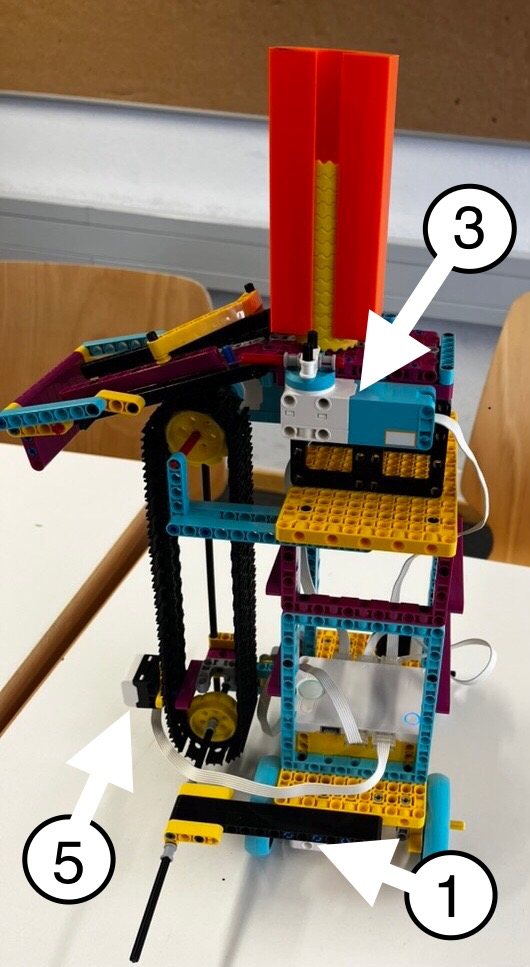
\includegraphics[width=0.5\linewidth]{images/188CF006-D571-4F2D-9337-8C4BDD7DAAEF_1_105_c}
	\caption{Seitenansicht links}
	\label{fig:188cf006-d571-4f2d-9337-8c4bdd7daaef1105c}
\end{figure}


\begin{figure}[H]
	\centering
	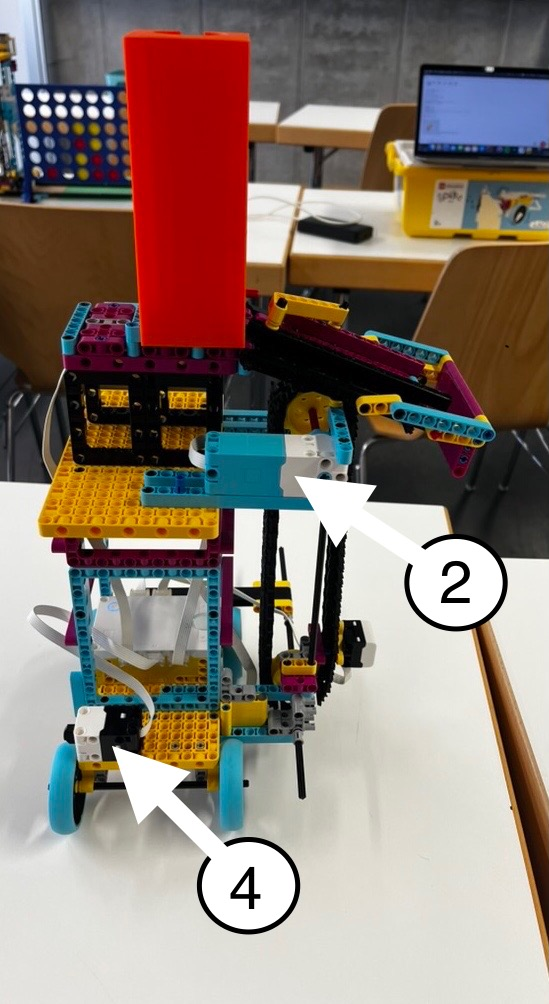
\includegraphics[width=0.5\linewidth]{images/DAE26A50-277E-4C6B-96A3-F2DE2CC9C004_1_105_c}
	\caption{Seitenansicht rechts}
	\label{fig:dae26a50-277e-4c6b-96a3-f2de2cc9c0041105c}
\end{figure}


\section{Software}
Im Kapitel Software wird genauer beschrieben, wie die Programmierung des Vier-Gewinnt-Roboters umgesetzt ist. Die Software bildet das Kernstück des Roboters und ist entscheidend dafür, dass dieser eigenständig am Spiel teilnehmen kann.

\begin{lstlisting}[language=Python]
	import motor
	import color_sensor
	import color
	import time
	import force_sensor
	from hub import port, sound
\end{lstlisting}

\begin{lstlisting}[language=Python]
	# --- CONFIGURATION ---
	my_piece = 1 # -1 = RED, 1 = YELLOW (AI player)
	opponent_piece = -my_piece
	
	speed_D = 230
	speed_A = 500
	speed_E = 600
	move_distance_e = 97 # Step motor E per row, calibrate if necessary!
	move_distance_d = 73
	break_motor_e = 1
	break_motor_e_back = 2
	break_motor_d = 1
	field_width = 7
	field_height = 6
	waiting_line = 1 # Waiting time after reaching the line (in seconds)
\end{lstlisting}


\begin{lstlisting}[language=Python]
	# --- HELPER FUNCTIONS ---
	def sensor_activated():
		try:   
			return force_sensor.force(port.C) > 30
		except:
			return False
	
	def update_board(row, col, detected_color):
		if detected_color in (color.RED, color.PURPLE, color.MAGENTA):
			board[row][col] = -1
		elif detected_color in (color.YELLOW, color.WHITE, color.GREEN):
			board[row][col] = 1
		else:
			board[row][col] = 0
	
	def print_board(board):
		symbol_map = {-1: "R", 1: "Y", 0: "B", None: "B"} 
		print("\nCurrent board (bottom right = [0][0]):")
		for row_idx in reversed(range(field_height)):
			row = board[row_idx]
			print(" ".join(symbol_map.get(cell, "?") for cell in row))
	
	def is_valid_location(board, col):
		return board[field_height-1][col] == 0
	
	def get_next_open_row(board, col):
		for r in range(field_height):
			if board[r][col] == 0:
				return r
			return None
	
	def winning_move(board, piece):
		for c in range(field_width-3):
			for r in range(field_height):
				if board[r][c] == piece and board[r][c+1] == piece and board[r][c+2] == piece and board[r][c+3] == piece:
					return True
		for c in range(field_width):
			for r in range(field_height-3):
				if board[r][c] == piece and board[r+1][c] == piece and board[r+2][c] == piece and board[r+3][c] == piece:
					return True
		for c in range(field_width-3):
			for r in range(field_height-3):
				if board[r][c] == piece and board[r+1][c+1] == piece and board[r+2][c+2] == piece and board[r+3][c+3] == piece:
				return True
			for r in range(3, field_height):
				if board[r][c] == piece and board[r-1][c+1] == piece and board[r-2][c+2] == piece and board[r-3][c+3] == piece:
			return True
	return False
	
	def evaluate_window(window, player):
		opp_player = opponent_piece if player == my_piece else my_piece
		score = 0
		if window.count(player) == 4:
			score += 100
		elif window.count(player) == 3 and window.count(0) == 1:
			score += 5
		elif window.count(player) == 2 and window.count(0) == 2:
			score += 2
		if window.count(opp_player) == 3 and window.count(0) == 1:
			score -= 4
		return score
	
	def evaluate(board):
		score = 0
		center_array = [board[r][field_width//2] for r in range(field_height)]
		center_count = center_array.count(my_piece)
		score += center_count * 3
		for r in range(field_height):
			row_array = [board[r][c] for c in range(field_width)]
			for c in range(field_width - 3):
				window = row_array[c:c+4]
				score += evaluate_window(window, my_piece)
				score -= evaluate_window(window, opponent_piece)
		for c in range(field_width):
			col_array = [board[r][c] for r in range(field_height)]
			for r in range(field_height - 3):
				window = col_array[r:r+4]
				score += evaluate_window(window, my_piece)
				score -= evaluate_window(window, opponent_piece)
		for r in range(field_height - 3):
			for c in range(field_width - 3):
				window = [board[r+i][c+i] for i in range(4)]
				score += evaluate_window(window, my_piece)
				score -= evaluate_window(window, opponent_piece)
		for r in range(3, field_height):
			for c in range(field_width - 3):
				window = [board[r-i][c+i] for i in range(4)]
				score += evaluate_window(window, my_piece)
				score -= evaluate_window(window, opponent_piece)
		return score
	
	transposition_table = {}
	
	def board_hash(board, maximizing_player):
		return (tuple([item for row in board for item in row]), maximizing_player)
	
	def get_dynamic_depth(board):
		# Count empty fields
		empty = sum(row.count(0) for row in board)
		if empty > 30:
			return 3 # Beginning: fast, low depth
		else:
			return 4 # End: high depth for best moves
		
	def alpha_beta(board, depth, alpha, beta, maximizing_player):
		key = (board_hash(board, maximizing_player), depth)
		if key in transposition_table:
			return transposition_table[key]
		valid_locations = [col for col in range(field_width) if is_valid_location(board, col)]
		valid_locations.sort(key=lambda c: abs(c - field_width // 2))
		terminal = winning_move(board, my_piece) or winning_move(board, opponent_piece) or len(valid_locations) == 0
		if depth == 0 or terminal:
			if terminal:
				if winning_move(board, my_piece): return (None, 1000000)
				elif winning_move(board, opponent_piece): return (None, -1000000)
				else: return (None, 0)
			else:
			return (None, evaluate(board))
		if maximizing_player:
			value = -float('inf')
			best_col = valid_locations[0]
			for col in valid_locations:
				row = get_next_open_row(board, col)
				if row is None:
					continue
				board_copy = [r[:] for r in board]
				board_copy[row][col] = my_piece
				new_score = alpha_beta(board_copy, depth-1, alpha, beta, False)[1]
				if new_score > value:
					value = new_score
					best_col = col
				alpha = max(alpha, value)
				if alpha >= beta:
					break
			result = (best_col, value)
		else:
			value = float('inf')
			best_col = valid_locations[0]
			for col in valid_locations:
				row = get_next_open_row(board, col)
				if row is None:
					continue
				board_copy = [r[:] for r in board]
				board_copy[row][col] = opponent_piece
				new_score = alpha_beta(board_copy, depth-1, alpha, beta, True)[1]
				if new_score < value:
					value = new_score
					best_col = col
				beta = min(beta, value)
				if beta <= alpha:
					break
			result = (best_col, value)
		transposition_table[key] = result
		return result
\end{lstlisting}

\begin{lstlisting}[language=Python]
	# --- MAIN PROGRAM ---
	board = [[0 for _ in range(field_width)] for _ in range(field_height)]
	last_board = [row[:] for row in board]
	
	def move_motor_e_to_zero():
		pass
	
	while True:
		print("Waiting for sensor at port C...")
		while not sensor_activated():
			time.sleep(0.1)
		print("Sensor detected! Starting move...")
		time.sleep(1)
		
		# Move to field
		motor.run_for_degrees(port.D, 198, 170)
		print("Field reached...")
		time.sleep(1.5)
		
		transposition_table.clear()
		
		opponent_piece_found = False
		opponent_col = None
		
		move_motor_e_to_zero()
		
		for col in range(field_width - 1, -1, -1):
			matrix_col = field_width - 1 - col
			if last_board[field_height-1][matrix_col] != 0:
				if col > 0:
					motor.run_for_degrees(port.D, move_distance_d, 170)
					time.sleep(break_motor_d)
				continue
		
		free_row = None
		for row in range(field_height):
			if last_board[row][matrix_col] == 0:
				free_row = row
				break
		if free_row is None:
			continue
		
		motor.run_for_degrees(port.E, move_distance_e * (free_row), speed_E)
		time.sleep(break_motor_e)
		time.sleep(waiting_line)
		
		detected_color = color_sensor.color(port.B)
		update_board(free_row, matrix_col, detected_color)
		print("Matrix entry: Row {}, Col {}: {}".format(
			free_row, matrix_col,
			"RED" if board[free_row][matrix_col] == -1
			else "YELLOW" if board[free_row][matrix_col] == 1
			else "NONE"))
		
		if (last_board[free_row][matrix_col] == 0 and
			board[free_row][matrix_col] == opponent_piece):
			print("New opponent piece in column {}, row {}".format(matrix_col, free_row))
			opponent_piece_found = True
			opponent_col = col
			time.sleep(1)
		
		motor.run_for_degrees(port.E, -move_distance_e * free_row, speed_E)
		time.sleep(break_motor_e_back)
		
		if opponent_piece_found:
			break
		
		if col > 0:
			motor.run_for_degrees(port.D, move_distance_d, speed_D)
			time.sleep(break_motor_d)
		
		if opponent_piece_found and opponent_col is not None and opponent_col != 0:
			steps_right = opponent_col
			motor.run_for_degrees(port.D, move_distance_d * steps_right, speed_D)
			time.sleep(4)
			
		board_numeric = [[0 if x is None else x for x in row] for row in board]
		dynamic_depth = get_dynamic_depth(board_numeric)
		best_col, _ = alpha_beta(
		board_numeric,
		depth=dynamic_depth,
		alpha=-float('inf'),
		beta=float('inf'),
		maximizing_player=(my_piece == 1)
		)
		
		best_row = get_next_open_row(board_numeric, best_col)
		color_str = "RED" if my_piece == -1 else "YELLOW"
		print("\nOptimal position for {}:".format(color_str))
		print("Column: {}, Row: {}".format(best_col, best_row))
		
		if best_col is not None and best_row is not None:
			physical_target_col = field_width - 1 - best_col
			motor.run_for_degrees(port.D, -move_distance_d * physical_target_col, speed_D)
			time.sleep(break_motor_d * 4)
			motor.run_for_degrees(port.A, -360, speed_A)
			time.sleep(3)
			board[best_row][best_col] = my_piece
			last_board = [row[:] for row in board]
			
			if winning_move(board, my_piece):
				print(" Congratulations! The robot has WON the game!")
				print_board(board)
				sound.beep(440, 1000000, 100)
				motor.run_for_degrees(port.D, -move_distance_d * best_col, speed_D)
				time.sleep_ms(2500)
				motor.run_for_degrees(port.D, -move_distance_d * 3, speed_D)
				sound.beep(0, 1000000, 100)
				break
		
			motor.run_for_degrees(port.D, -move_distance_d * best_col, speed_D)
		
		print_board(board)
		time.sleep_ms(2500)
		motor.run_for_degrees(port.D, -199, speed_D)
		
		time.sleep(break_motor_d)
		
		while sensor_activated():
			time.sleep(0.1)
		print("Move completed. Waiting for next activation...")
	
	
\end{lstlisting}

